\section{Pistepilvien visualisointiin käytetyt tietorakenteet}\label{kirjallisuus}

Edellä mainittuihin haasteisiin on otettu kantaa laajalti alan julkaisuissa. Lupaavin tekniikka tarkkuustasojen muodostamiseen, ulkoisen muistin käyttöön ja pistepilvien harventamiseen näyttää olevan pistepilven jakaminen hierarkiseen tietorakenteeseen. Ajatuksena on, ettei kaikkia pisteitä tarvitse käydä läpi jokaisella ruudunpäivityksellä, vaan hierarkian yläpäässä on karkein tarkkuustaso ja alaspäin kulkiessa tarkkuus kasvaa. Hierarkiasta voidaan joko valita tarkkuustaso, joka takaa nopean ruudunpäivityksen tai tarkentaa kuvaa inkrementaalisesti, kunnes renderöintiaika loppuu kesken tai katselupiste siirtyy ja pistepilvi täytyy renderöidä uudestaan toisesta kuvakulmasta. 

Esitellään seuraavaksi muutama kiinnostava hierarkinen tietorakenne. Aihealueen pioneerityönä pidetään Rusinkiewiczin ja Levoyn vuonna 2000 julkaisemaa Qsplatia \cite{qsplat}, joka onkin antanut paljon vaikutteita uudemmille tietorakenteille. Dachsbacher et al. esittelivät peräkkäispistepuut \cite{spt}, jotka voidaan renderöidä hyvin nopeasti näytönohjaimella. Viime vuosina pistepilvien visualisoinnin tutkimuksen kirkkainta kärkeä on edustanut Wienin teknillisen yliopiston tietokonegrafiikan tutkimusyksikkö. Tämän tutkielman päälähteinä käytetään Claus Scheiblauerin ja Markus Schützin julkaisuja sisäkkäispistepuista \cite{scheiblauer},\cite{potree}. Schütz et al. ovat esitelleet myös joitakin mielenkiintoisia, ei-hierarkisia tekniikoita \cite{clod}, jotka kuitenkin rajoittuvat näytönohjaimen muistiin mahtuviin pistepilviin.

Luvun lopussa listataan laitossuunnitteluohjelmiston asettamia vaatimuksia pistepilvivisualisoijan käyttämälle tietorakenteelle ja todetaan sisäkkäispistepuiden vaikuttavan lupaavilta myös laitossuunnitteluohjelmistossa käytettäväksi. 

\subsection{QSplat}
Yksi ensimmäisistä pistedatan visualisointiin käytetyistä hierarkisista tietorakenteista on Rusinkiewiczin ja Levoyn esittämä QSplat, joka on kehitetty kolmioverkon visualisointiin pisteiden avulla. Tietorakenne muodostaminen vaatii, että mallin kolmioiden normaalivektorit tunnetaan, joten se ei suoraan sovellu raa'an pistepilvidatan käsittelyyn.\footnote{Itse asiassa Rusinkiewicz ja Levoy käyttivät laserkeilatusta pistepilvestä muodostettua kolmioverkkoa, jonka tietorakenne esitti yksinkertaistettuna pistedatana.} QSplatissa on käytetty kuitenkin monia kiinnostavia tekniikoita, joita voi hyödyntää pistepilvidatan käsittelyssä. \cite{qsplat}

QSplat perustuu puurakenteeseen, jonka solmuissa on rajauspalloja \engl{bounding sphere}. Pallot jakavat avaruutta rekursiivisesti pienempiin osiin siten, että juuren pallo sisältää kaikki mallin kolmiot ja jokainen sisäsolmu jakaa avaruuden keskimäärin neljään osaan. Puun latva saavutetaan, kun avaruuden jakamisen seurauksena jäljelle jää yksi kolmio. Jäljelle jäävästä kolmiosta muodostetaan lehtisolmu, jonka rajauspallo sisältää koko kolmion. Puun visualisointi onnistuu piirtämällä jokaisen pallon kohdalle sopivan kokoinen täplä \engl{splat}. Puurakenne mahdollistaa myös tehokkaan pisteiden karsimisen niiden näkyvyyden perusteella. Jos solmun rajauspallo ei ole näkökentässä, eivät sen lapsetkaan ole ja haaraan läpikäyntiä ei tarvitse jatkaa. \cite{qsplat}

Puurakenne tallennetaan levylle leveysjärjestyksessä \engl{breadth-first}. Tämän ansiosta puun tasot muodostavat luonnolliset tarkkuustasot: juurisolmun rajauspallo esittää koko mallia, ensimmäinen taso sisältää muutaman pienemmän pallon, ja niin edelleen. Kun tällainen tiedoston sisäinen rakenne yhdistetään ulkoisen muistin tekniikoihin, voidaan täplien piirtäminen aloittaa heti, kun tarpeeksi puun solmuja on ladattu levyltä muistiin. Puuta käydään läpi kunnes solmujen rajauspallot ovat niin pieniä, ettei niiden kohdalle enää kannata piirtää täpliä. Puun rakennetta on havainnollistettu kuvassa \ref{tarkkuustasot}. \cite{qsplat}

\begin{figure}
    \centering
    \subfile{fig/puuntasot.tex}
    \caption{QSplatin käyttämän pallopuun läpikäyminen taso kerrallaan muodostaa luonnolliset tarkkuustasot}
    \label{tarkkuustasot}
\end{figure}

Toinen hyödyllinen QSplatissa käytetty tekniikka on koordinaattien kvantisointi \engl{quantization}. Kun tarkkuudesta voidaan tinkiä, solmujen rajauspallojen absoluuttisia koordinaatteja ei tallenneta, vaan niiden sijainti ilmaistaan suhteessa vanhempiinsa. Pallon säteen ja keskipisteen suhteellisen poikkeaman ilmaisemiseen käytetään vain 13:a arvoa. Pallon säde $r$ voi olla välillä $[\frac{1}{13}, \frac{13}{13}]$ ja samaten keskipisteen suhteellisen poikkeaman $x, y$ ja $z$ -koordinaatit ovat vanhemman pallon läpimitan kolmastoistaosan monikertoja. Kun vielä hylätään vanhemman pallon ulkopuolella olevat keskipisteet ja käytetään hakutaulua, voidaan pallon sijainti esittää vain 13:lla bitillä, kun normaali liukulukuesitys vaatisi vähintään 16 tavua. \cite{qsplat}

QSplat onnistui renderöimään 1,5-2,5 miljoonaa pistettä sekunnissa, mikä on sen aikaisella laitteistolla erinomainen tulos \cite{qsplat}. Kuten sanottu, se ei sellaisenaan kuitenkaan sovellu laserkeilattujen pistepilvien käsittelyyn. Pistepilvien pisteiden normaaleja ei yleensä tiedetä, joten ne pitäisi esiprosessointivaiheessa selvittää esimerkiksi luvussa \ref{workflow} esitetyllä tekniikalla. 

Toisena ongelmana voidaan pitää tapaa, jolla mallin kolmioita esitetään palloina. Tietorakenteeseen luodaan nimittäin uutta dataa, kun lehtisolmuihin tallennettujen, yhden kolmion sisältävien pallojen lisäksi ylemmillä tasoilla on keinotekoisia, monia kolmioita kuvaavia palloja. QSplat tarjoaa kuitenkin monia tekniikoita, joita pistepilviä käsittelevässä tietorakenteessa voidaan hyödyntää, kuten hierarkinen rakenne ja koordinaattien suhteellinen esitystapa.

\subsection{Peräkkäispistepuut}
Dachsbacher et al. esittelevät niin kutstutun peräkkäispistepuun \engl{sequential point tree}, joka yrittää hyödyntää QSplatin hierarkian lisäksi näytönohjaimen laskentatehoa. Dachsbacher et al. litistävät hierarkian yksiulotteksi taulukoksi, joka voidaan ladata näytönohjaimen muistiin. Renderöintivaiheessa näytönohjaimen riittää vain valita mitkä osat taulukosta pirretään ruudulle. Peräkkäispistepuut siirtävät siis työtä näytönohjaimelle ja jättävät suorittimen vapaaksi muuta laskentaa varten. \cite{spt}

Peräkkäispistepuita on käytetty kuvaamaan yksittäisiä objekteja isommassa mallissa. Jokaisesta objektista näytteistetyt pisteet järjestetään pallopuuhun samaan tapaan kuin QSplatissa. Pisteet sijaitsevat puun lehtisolmuissa, joiden rajauspallot ovat lähes yhtäsuuria ja sisäsolmut kuvaavat lapsiensa unionia siten, että niiden rajauspallo juuri ja juuri peittää lastensa pallot. Visualisointiin käytetään rajauspallojen kokoisia täpliä joiden väri määräytyy puun haaran alempien solmujen värien keskiarvolla. \cite{spt}

Jokaiselle solmulle lasketaan virhe $e$ sen perusteella, kuinka hyvin sen rajauspallo peittää lapsisolmujensa rajauspallot. Ajatuksena on käydä hierarkiaa läpi syvemmälle, jos $e/r < \epsilon$, missä $r$ on etäisyys katselupisteestä solmuun ja $\epsilon$ käyttäjän asettama arvo. Tästä johdetaan katseluetäisyydelle rajat $r_{min}$ ja $r_{max}$, joiden välillä solmu valitaan renderöitäväksi. Renderöintivaiheessa hierarkia litistetään taulukoksi ja pisteet järjestetään solmujen $r_{max}$-arvon mukaan, jonka jälkeen ne ladataan näytönohjaimen muistiin. Näin näytönohjaimen täytyy käydä taulukkoa läpi vain siihen asti, kun katselupisteen etäisyys $r$ ylittää käsiteltävän pisteen $r_{max}$-arvon. \cite{spt}

Peräkkäispistepuut voidaan renderöidä nopeasti näytönohjaimen tehokkaan käytön ansiosta, mutta niissä on myös heikkouksia. Tietorakenteen vaatimuksena on, että kaikki data mahtuu näytönohjaimen muistiin. Näin on näytönohjaimesta riippuen vain pienillä malleilla ja tilannetta pahentaa se, että peräkkäispistepuut eivät ole kovin säästäväisiä muistin suhteen. Hierarkian jokaisessa sisäsolmussa luodaan QSplatin tapaan lisää dataa, kun lapsisolmujen unionia kuvataan uudella täplällä, jolle tarvitsee tallentaa sijainti, koko ja väri.

Wimmer ja Scheiblauer esittävät parannuksia peräkkäispistepuihin muistioptimoiduilla peräkkäispistepuilla \engl{memory optimized sequential point tree, MOSPT}. Uusien täplien luomisen sijaan puun sisäsolmuissa valitaan lapsisolmuista edustaja, joka parhaiten kuvaa sisäsolmusta alkavaa haaraa. Haaran solmujen väreistä laksetaan keskiarvo ja edustajasolmuksi valitaan sellainen, jonka väri on lähinnä keskiarvoa. Olemassa olevien solmujen käyttäminen tarkkuustasojen muodostamiseen on tärkeä oivallus, sillä käsiteltäessä massiivisia pistepilviä tulisi välttää ylimääräisen datan luomista. \cite{ip}

Wimmer ja Scheiblauer määrittävät solmun virheeksi yksinkertaisesti rajauspallon halkaisijan, minkä johdosta kunkin tason jokaisella solmulla on samat $r_{min}$ ja $r_{max}$ -arvot. Tämän vuoksi renderöintivaiheessa ei tarvitse tarkastaa jokaisen solmun $r_{max}$ arvoa, vaan riittää tietää, mistä pistetaulukon indeksistä alkaa mikäkin hierarkian taso. Tämän jälkeen taulukosta renderöidään pisteitä kunnes saavutetaan taso, jolla rajauspallot projisoituisivat alle pikselin kokoisiksi kuvaruudulle. \cite{ip}

%Kun hierarkiaa litistetään taulukoksi, ei edustajasolmuja tarvitse tarvitse lisätä 

 %Kun hierarkian läpikäymistä jatketaan niin pitkälle, että solmujen täplät ovat yhden pikselin kokoisia, ei lopputulokseen jää aukkoja. \cite{ip}

\subsection{Sisäkkäispistepuut}\label{sisäkkäis}

\begin{figure}
    \centering
    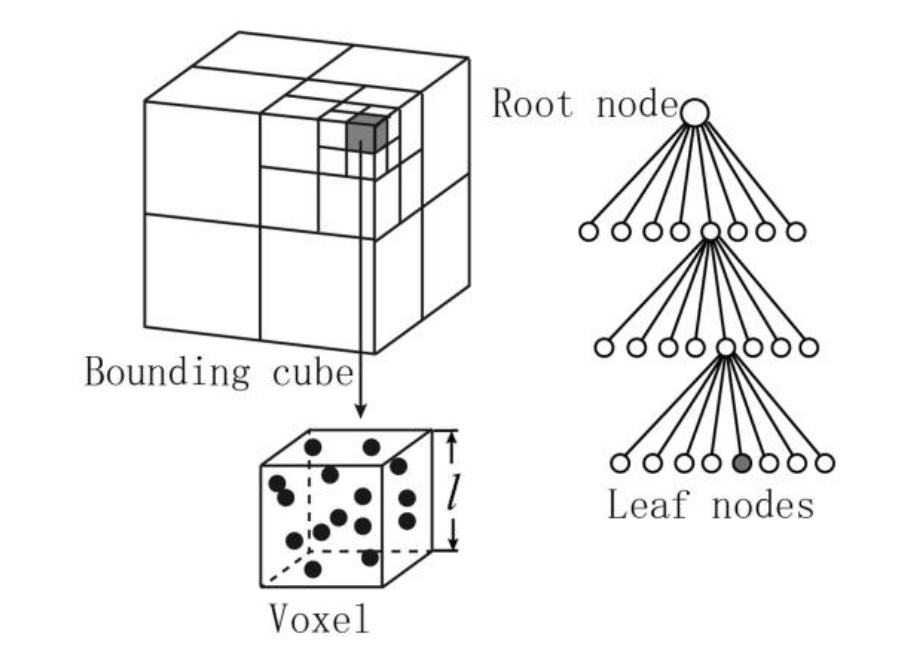
\includegraphics[width=0.5\paperwidth]{img/octree.png}
    \caption{Oktettipuun juurisolmu sisältää kaikki pisteet sisältävän rajauslaatikon. Jokainen sisäsolmu jakaa rajauslaatikkonsa kahdeksaan osaan. \cite{octreekuva}}
    \label{img:octree}
\end{figure}

Wimmer ja Scheiblauer kritisoivat muistioptimoituja peräkkäispistepuita siitä, että ne eivät tue näkökentän ulkopuolisten pisteiden tehokasta karsimista ja siitä, ettei muistioptimointi yksinään riittänyt poistamaan tarvetta ulkoisen muistin algoritmeille. Ratkaisuksi he esittivät sisäkkäisiä oktettipuita \engl{nested octree}. Oktettipuu\footnote{Tätä suomennosta käyttää esimerkiksi Davidsson \cite{oktettipuu}. Vaihtoehtoinen suomennos on kahdeksanpuu.} on yksinkertainen avaruutta rekursiivisesti jakava tietorakenne, jonka jokainen sisäsolmu jakaa kuvaamansa avaruuden kahdeksaan samankokoiseen osaan. Oktettipuun rakennetta on havainnollistettu kuvassa \ref{img:octree}. 

Wimmerin ja Scheiblauerin tietorakenteessa oktettipuita on kahdessa tasossa. Ulompaa oktettipuuta käytetään avaruuden jakamiseen, sen tehokkaseen läpikäymiseen ja näkökentän ulkopuolisten alueiden karsimiseen. Ulomman puun jokainen solmu sisältää yhden sisemmän oktettipuun, joka vastaa samaa avaruuden osaa, kuin ulkoisen puun solmu. Pisteet sijoitetaan sisempiin puihin, yksi jokaiseen solmuun. \cite{ip}

\begin{figure}
    \centering
    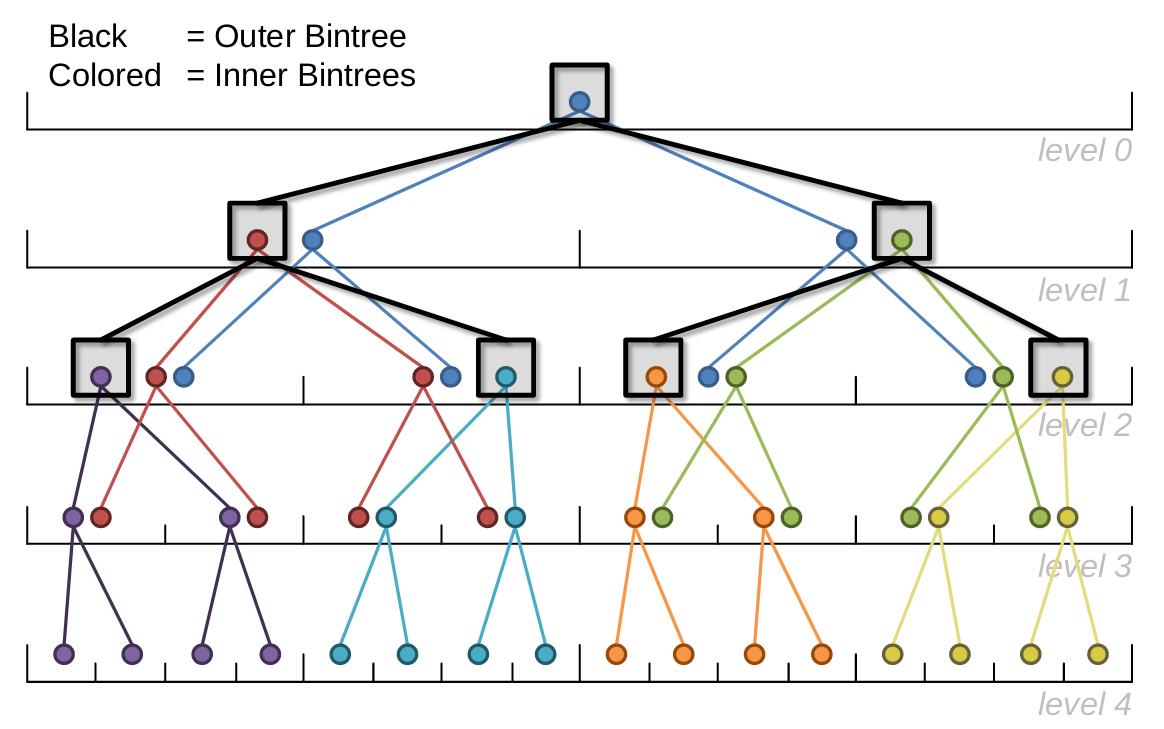
\includegraphics[width=0.6\paperwidth]{img/nested.png}
    \caption{Sisäkkäinen binääripuu, jossa sekä ulomman, että sisempien puiden syvyys on kolme. Ulompaa puuta kuvaavat mustat neliöt ja sisempää värikkäät ympyrät. Puista muodostuu viisi tarkkuustasoa. \cite{scheiblauer}}
    \label{nested}
\end{figure}

Sisäkkäisistä oktettipuista luodaan tarkkuustasot siten, että sisemmistä puista kerätään pisteitä ulomman puun tasojen mukaan. Tarkkuustasoon kuuluvat pisteet sijaitsevat siis ulomman puun samalla tasolla, mutta useiden sisempien puiden eri tasoilla. Tarkkuustasojen muodostumista on havainnollistettu kuvassa \ref{nested}. Puut tallennetaan levylle tarkkuustaso kerrallaan, mikä mahdollistaa ulkoisen muistin algoritmien käytön. Visualisoitaessa tarvitsee levyltä lukea pisteitä vain haluttuun tarkkuustasoon asti, eikä loppuja pisteitä tarvitse ladata muistiin. \cite{ip}

Scheiblauer jalostaa sisäkkäisten oktettipuiden ideaa väitöskirjassaan esittelemällä muokattavat sisäkkäiset oktettipuut \engl{modifiable nested octree, MNO}. Jos edellä esiteltyjä sisäkkäisiä oktettipuita halutaan muokata rakentamisen jälkeen, on sisemmät puut rakennettava ja muokattu hierarkia tallennettava levylle uudestaan. Nimensä mukaisesti MNO mahdollistaa tehokkaan pisteiden lisäämisen ja poistamisen. \cite{scheiblauer}  

MNO:n rakenne eroaa sisäkkäisistä oktettipuista siten, että sisemmät puut korvataan säännöllisillä kolmiulotteisilla ruudukoilla, joihin pisteet tallennetaan. MNO:n rakentaminen alkaa juurisolmusta, joka vastaa kaikki pisteet peittävää avaruutta. Solmun sisältämä ruudukko jakaa solmua kuvaavan avaruuden osan $128^3 = 2 097 152$ soluun. Pisteitä lisätään puuhun yksi kerrallaan niin, että jokaiseen ruudukon soluun mahtuu vain yksi piste. Jos solu on varattu, sijoitetaan piste ylimääräiseen taulukkoon odottamaan, että vastaavia pisteitä kertyy tarpeeksi, jotta olisi järkevää luoda uusia solmuja puuhun. Kun ennaltamäärätty vähimmäismäärä pisteitä on kertynyt ylimääräisten pisteiden taulukkoon, luodaan ruudukon sisältävälle solulle lapsisolmuja ja sijoitetaan ylimääräiset pisteet niihin. Ruudukkoon sijoitettavien pisteiden määrälle on hyvä asettaa myös yläraja. \cite{scheiblauer}

Jokainen tietorakenteen solmu tallennetaan omaan tiedostoonsa levylle, josta niitä ladataan muistiin visualisointivaiheessa tarvittaessa. Renderöintialgoritmiin kuuluu käyttäjän asettama pistebudjetti, joka asettaa ylärajan yhdessä ruudunpäivityksessä piirrettävien pisteiden määrälle.\footnote{Scheiblauer testasi pistepilvivisualisoijaansa asettamalla rajan vain sataantuhanteen pisteeseen.} Tätä rajaa säätämällä käyttäjä saa jonkinlaisen kontrollin ruudunpäivitystaajuuden suhteen. \cite{scheiblauer}

Tiedostorakenne mahdollistaa hierarkian tehokkaan muokkaamisen. Lisättäessä uusia pisteitä MNO:hon tarkastetaan ensin, sijoittuuko se juurisolmun kuvaamaan avaruuden osaan. Jos näin on, onnistuu lisääminen kuten rakennusvaiheessa. Muussa tapauksessa juurisolmulle luodaan vanhempia kunnes jokin niistä muodostaa tarvittavan kokoisen avaruuden, ja piste lisätään sen ruudukkoon. Kun puun vanhan juuren yläpuolelle luodaan uusia solmuja, jää niiden ruudukot vajaaksi. Tällöin alemmista solmuista nostetaan pisteitä ylöspäin niin kauan, kunnes vajaita ruudukoita on vain lehtisolmuissa. Pisteiden poistaminen puusta on triviaalia, kun sisäsolmuihin mahdollisesti jäävät tyhjät ruudukot täytetään kuten pisteitä lisättäessä. \cite{scheiblauer}

Scheiblauer oli ottanut MNO:ta kehittäessään vaikutteita Michael Wandin et al. esittämästä oktettipuusta, jonka sisäsolmuihin kuuluu myös ruudukko. Pisteet tallennetaan kuitenkin ruudukon sijaan lehtisolmuihin joihin mahtuu kuhunkin enintään satatuhatta pistettä. Sisäsolmuissa pidetään kopiota yhdestä niiden läpi kulkeneesta pisteestä ja tarkkustasot muodostetaan näistä sisäsolmujen pisteistä. Wandin et al. tietorakenne käyttää MNO:n tapaan ulkoista muistia ja mahdollistaa tehokkaat lisäys- ja poisto-operaatiot. \cite{wand}

Markus Schütz jatkoi Wimmerin ja Scheiblauerin työtä esittelemällä opinnäytetyössään verkkoselaimessa ajettavan Potree-nimisen pistepilvivisualisoijan. Potreen käyttämä tietorakenne perustuu Scheiblauerin muokattaviin sisäkkäisiin oktettipuihin, mutta hierarkian rakennusvaiheessa kiinnitetään huomiota pisteiden tasaiseen jakautumiseen solmujen välille. Oktettipuun sisäsolmujen ruudukoihin hyväksytään uusia pisteitä vain, jos ne ovat tarpeeksi kaukana muista ruudukon pisteistä. Lehtisolmut hyväksyvät ennaltamäärättyyn rajaan saakka kaikki pisteet, kunnes ne muutetaan sisäsolmuiksi ja liian lähekkäin olevat pisteet jaetaan uusien lapsisolmujen kesken. \cite{potree}

Potree käyttää ulkoista muistia tehokkaasti ja pystyy käsittelemään jopa 640 miljardia pistettä sisältäviä pistepilviä.\footnote{Kyseinen pistepilvi (Actueel Hoogtebestand Nederland, ANH2, \url{http://ahn2.pointclouds.nl/}) kuvaa koko Alankomaiden valtiota ja se vaatii 7,68 teratavua tallennustilaa. Potreen tietorakenteessa pistepilvi jakautui 13:lle tasolle ja 38:aan miljoonaan solmuun.} Rakennusvaiheessa oktettipuun solmuja tallennetaan tasaisin väliajoin levylle, jottei muisti täyttyisi. Kun jokainen solmu tallennetaan omaan tiedostoonsa, on yksittäisten solmujen tallentaminen ja lukeminen levyltä helppoa. Massiivisia pistepilviä kuvaavat hierarkiatkin voivat olla satojen megatavujen kokoisia. Schütz ratkaisee suurten hierarkioiden nopean lataamisen verkon yli jakamalla senkin puurakenteeseen. Näin voidaan välttää sekä turhien pisteiden, että näkökentän ulkopuolella olevien hierarkian haarojen lataaminen muistiin. \cite{potree}

Potreen visualisointialgoritmi priorisoi niitä hierarkian solmuja, jotka ovat lähellä katselupistettä ja joiden kuvaruudulle projisoitu koko on suurin. Renderöinnin suorituskykyä voidaan säädellä Scheiblauerin toteutuksen mukaisesti käyttäjän asettamalla pistebudjetilla. Schütz on kehittänyt Potreehen myös näytönohjaimella ajettavan algoritmin mukautuvaan pisteiden koon määrittämiseen; pistepilven harvemmissa osissa piirretään pisteet suurempina, jottei reikiä esiintyisi. \cite{potree}

\subsection{kd-puut}
Suosittujen oktettipuiden lisäksi on pistepilvien visualisoinnissa käytetty kd-puita \engl{k-dimensional tree, kd-tree}\footnote{Kolmiulotteisten mallien visualisointiin käytetyissä kd-puissa luonnollisesti $k=3$.}. Oktettipuusta poiketen kd-puut eivät jaa pistepilveä yhtäsuuren tilavuuden omaaviin osiin, vaan jokainen solmu jakaa kuvaamansa alueen kahtia niin, että tilanjakotason molemmille puolille jää yhtä monta pistettä. Tätä varten pisteet on järjestettävä, mikä pidentää puun rakennusaikaa. Toisaalta tietorakenteen siirtely kiintolevyltä muistiin ja sieltä näytönohjaimelle on helpompaa, kun puu on tasapainoinen, eli kaikki solmut ovat saman kokoisia. \cite{richter}

Richter et al. kehittivät massiivisten ulkoilmakeilausten visualisointiin kd-puuhun perustuvan pistepilvirenderöijän, joka käytti luokiteltua pistepilvidataa. Pisteet oli jaettu objektiluokkiin, kuten kasvillisuus, vesi tai rakennus, joille jokaiselle rakennettiin oma kd-puu. Renderöintivaiheessa kd-puista lähetetään solmuja näytönohjaimelle niiden kuvaruudulle projisoidun koon määräämässä järjestyksessä niin, että jokaisella objektiluokalla oli oma rajansa muistinkäytölle. \cite{richter}

Futterlieb et al. käyttivät samankaltaista kd-puuta luokittelemattomalle pistedatalle. Edellä mainitusta toteutuksesta poiketen tarkkuustaso valitaan etsimällä puusta yksi taso, jolta saadaan renderöityä sopiva määrä pisteitä. Varmistaakseen, että ruudulle saadaan aina jonkinlainen tarkkuustaso renderöityä nopeasti Futterlieb et al. pitivät kahta miljoonaa pistettä näytönohjaimen muistissa jatkuvasti riippumatta siitä, olivatko ne näkyvissä. \cite{smooth}

\subsection{Ei-hierarkiset tekniikat}

Pistepilvistä voi muodostaa tarkkuustasoja myös ilman hierarkista tietorakennetta. Markus Schütz et al. \cite{clod} esittivät virtuaalitodellisuuslaseille suunnatun pistepilvirenderöijän, joka hierarkian muodostamisen sijaan käy koko pistepilveä läpi ja muodostaa siitä noin viiden ruudun välein uuden, sopivan tiheästi näytteistetyn osajoukon. Tämä jatkuviksi tarkkuustasoiksi \engl{continuous LOD} kutsuttu tekniikka ei siis jaa pisteitä tietorakenteen solmuihin, joilla on diskreetit tarkkuustasot, vaan pisteiden etäisyys toisistaan vaihtelee sen perusteella, kuinka kaukana ne ovat kamerasta. \cite{clod}

\begin{figure}
    \centering
    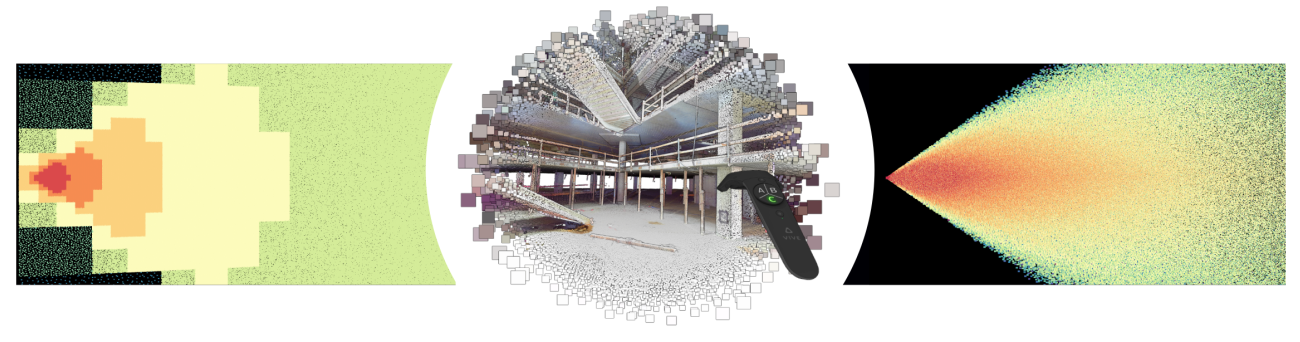
\includegraphics[width=\textwidth]{img/clod.png}
    \caption{Vasemmalla pistepilvi on jaettu diskreetteihin tarkkuustasoihin, joiden välillä on selkeät rajat. Oikealla on käytetty jatkuvia tarkkuustasoja ja pisteet sulautuvat siististi kuvaan. \cite{clod}}
    \label{img:clod}
\end{figure}

Jatkuvat tarkkuustasot ratkaisevat hierarkisia tietorakenteita käytettäessä usein esiintyvän ongelman diskreettien tarkkuustasojen näkyvistä rajoista. Renderöidyssä kuvassa ei näy selkeitä eroja matalalla ja korkeammalla tarkkuudella renderöityjen solmujen välillä kun tarkkuus laskee vähitellen kamerasta poispäin. Kuvassa \ref{img:clod} vasemmalla on havainnollistettu diskreettejä tarkkuustasoja ja oikealla jatkuvia tarkkuustasoja.

Schütz et al. \cite{progressive} esittelivät hiljattain myös toisen ei-hierarkisen tekniikan. Pisteitä ladataan näytönohjaimelle, joka asettaa niitä verteksipuskureihin satunnaisessa järjestyksessä. Pisteiden renderöiminen aloitetaan heti kun riittävä määrä pisteitä on saatu ladattua ja kuvaa tarkennetaan seuraavilla ruuduilla samalla kun näytönohjaimen muistiin ladataan lisää pisteitä. Puskurien täyttäminen satunnaisessa järjestyksessä saa aikaan kuvan miellyttävän tarkentumisen.

Nämä kaksi ei-hierarkista tekniikkaa toimivat vain silloin, kun pistepilvet mahtuvat kokonaisuudessaan näytönohjaimen muistiin. Tämä on kuitenkin vähenevissä määrin rajoittava tekijä, sillä uusimmissa näytönohjamissa voi olla jopa 48 gigatavua muistia, johon mahtuu jo erittäin suuria pistepilviä \cite{rtx}. Laitossuunnitteluohjelmistossa käytettävien pistepilvien kokoluokka on harvoin teratavuja, joten voisi olla kannattavaa hierarkisten tietorakenteiden kehittämisen sijaan keskittyä harventamaan pistepilveä niin, että se mahtuu näytönohjaimen muistiin ja käyttää jotakin tekniikkaa, joka käyttää näytönohjaimen rinnakkaislaskentatehoa mahdollisimman tehokkaasti.

\subsection{Laitossuunnitteluohjelmistoon soveltuva tietorakenne}\label{usecase}

Laitossuunniteluohjelmisto esittää pistepilvivisualisoijan käyttämälle tietorakenteelle tiettyjä vaatimuksia. Selvitetään näitä vaatimuksia käyttötapausten perusteella. Kaksi yleistä käyttötapausta pistepilvien kanssa työskenneltäessä ovat mallintaminen ja katselu. 

Kun laitoksesta halutaan luoda ajantasalla oleva 3d-malli pistepilven avulla, täytyy se mallintaa suunnitteluohjelmiston käyttämäksi geometriaksi pistepilveä mukaillen. Lattiat ja seinät on tasoina helppo asettaa paikalleen, kuten myös suunnitteluohjelmiston komponenttikirjastosta löytyvät laitteet. Suurin työ on yleensä putkistoissa, ilmakanavissa ja kaapeliradoissa. Useat suunnitteluohjelmistot tarjoavat jonkinasteista automatisointia etenkin putkien reititykseen pistepilven päälle. Ohjelmisto voi automaattisesti tunnistaa pilvestä sylintereitä ja asettaa niiden päälle sopivia putkisto-osia. Vaihtoehtoisesti käyttäjä voi valita pilvestä muutamia pisteitä ja ohjelmisto laskee niiden perusteella putken pituuden ja halkaisijan ja asettaa oikean osan paikalleen. Mallinnustyö ja etenkin automaattiset muodontunnistusalgoritmit asettavat ohjelmistolle vaatimuksen tarkkuudesta. Laitossuunnitteluohjelmistossa käytetään yleensä millimetrejä perusyksikköinä, joten pistepilvessä ei saisi esiintyä senttimetrien virheitä.

Mallintamisessa tärkeässä roolissa on suunnittelijan käyttämät näkymät ja pistepilven rajaaminen. Yleensä suunnittelija käyttää muutamaa koordinaattiakselien suuntaista näkymää samanaikaisesti, jotta kursorin saa helposti oikeaan paikkaan. Näkymän syvyys asetetaan usein hyvin pieneksi, jotta mallista näkyisi vain kulloisenkin mallinnustyön vaatima pieni siivu. Myös pistepilveä voidaan rajata niin, että siitä näkyy vain tarpeellinen osa. Pistepilviä visualisoivan ohjelmiston tulisi siis kyetä rajaamaan pilveä toistuvasti ja nopeasti. Käyttökokemus olisi paras, jos käyttäjä pystyisi hiirellä interaktiivisesti määrittämään tilan, jonka sisäpuolella olevat pisteet renderöitäisiin. Lisäksi pistepilvi tulee voida renderöidä useaan eri näkymään samanaikaisesti.

Mallinnustyössä käytetään usein hyväksi mittaustyökalua. Pistepilviä käytetään usein tarkastamaan, mahtuuko laitokseen jokin uusi laite tai putkisto. Tällöin on hyödyllistä suorittaa mittauksia joko kahden pistepilven pisteen, tai pisteen ja 3d-mallin geometrian välillä. Mittausoperaatiossa käyttäjä valitsee pistepilvestä kursorilla haluamansa pisteen ja ohjelmisto palauttaa lähimmäksi kursoria projisoidun pisteen. Käyttäjän kannalta olisi miellyttävää, jos mittausoperaatioita tehtäessä ei tarvitsisi odottaa, kun pistepilven miljoonien pisteiden joukosta etsitään juuri kursorin alla oleva piste. Yksittäisten pisteiden hakeminen pilvestä täytyy siis olla nopeaa.

Toinen yleinen pistepilvien käyttökohde on 3d-mallin katselu joko laitossuunnitteluohjelmistossa tai erityisessä mallinkatseluohjelmistossa. Etenkin suunnitteluprojektien esimiehet haluavat usein tarkastella suunnittelijoiden luomaa 3d-mallia helposti ja nopeasti. Luonnollisesti malliin kuuluvat pistepilvet tulevat myös näkyä katselijalle. Tämä saattaa tuottaa haasteita ohjelmiston kannalta, sillä katseluohjelmistojen käyttäjillä on käytettävissä harvoin yhtä järeää laitteistoa, kuin suunnittelijoiden työasemat. Mallinkatseluohjelmistossa pistepilveä harvemmin rajataan pienemmäksi, joten renderöitäviä pisteitä on niin paljon, etteivät ne mahdu kerralla keskusmuistiin tai näytönohjaimen muistiin. Yleensä käyttäjä myös liikuttaa näkymää mallin ympäri enemmän kuin mallinnustyössä, joten pistepilvivisualisoinnin suorituskyky ja tarkkuustasot ovat entistäkin tärkeämpiä.

Tässä tutkielmassa kehitetään laitossuunnitteluohjelmistolle optimoitu hierarkinen tietorakenne pistepilvien käsittelyyn. Esitetään tälle tietorakenteelle seuraavat vaatimukset edellä mainittujen käyttötapausten perusteella:
\begin{enumerate}
    \item \label{vaatimus:lod} On voitava visualisoida karkea yleiskuva pistepilvestä vain pienellä osalla datasta. 
    \item \label{vaatimus:ooc} On käytettävä ulkoisen muistin algoritmeja, eli koko pilveä ei pidetä kerralla keskusmuistissa.
    \item \label{vaatimus:harvennus} Pistepilven vaatimaa tallennustilan määrää voidaan laskea harventamalla sen tiheästi näytteistettyjä osia. 
    \item \label{vaatimus:crop} Käyttäjän on voitava määrittää pilvestä alueita, joiden sisältävien tai ulkopuolelle jäävien pisteiden ominaisuuksia, kuten näkyvyyttä tai väriä, voidaan muuttaa.
    \item \label{vaatimus:select} Pilvestä on voitava nopeasti ja tarkasti valita yksittäisiä pisteitä.
    \item \label{vaatimus:virhe} Pistepilvessä ei saa esiintyä yli millimetrin suuruisia virheitä.
\end{enumerate}

Luvussa \ref{sisäkkäis} esitelty Potree on osoittaunut massiivisten pistepilvien interaktiivisen visualisoinnin olevan mahdollista jopa verkkoselaimessa, jossa etenkin tiedonsiirtonopeus rajoittaa renderöinnin nopeutta. Tarkastellaan siis sisäkkäispistepuiden sovelutuvuutta laitossuunnitteluohjelmistoon. 

Oktettipuun läpikäyminen taso kerrallaan muodostaa tehokkaasti tarkkuustasot, joten vaatimus \ref{vaatimus:lod} on helppo tyydyttää. Pisteiden asettelu sisäkkäisten oktettipuiden solmuihin mahdollistaa myös vaatimuksen \ref{vaatimus:ooc} mukaisesti ulkoisen muistin käyttämisen. Scheiblauerin muokattavien sisäkkäisten oktettipuiden jokainen solmu sisältää ruudukon, johon pisteet sijoitetaan. Mitä syvemmällä tasolla solmu on, sitä pienempiä ruudukon solut ovat. Vaatimuksen \ref{vaatimus:harvennus} esittämä pilven harvennus onnistuu asettamalla puulle enimmäissyvyys ruudukon koon mukaan ja hylkäämällä lehtisolmuissa kaikki pisteet, jotka tulisi lisätyksi jo varattuun soluun. 

Valintaoperaatiot onnistuvat nopeasti oktettipuussa. Puun jokainen solmu sisältää tiedon sen sisältämien pisteiden rajauslaatikosta \engl{bounding box}, joten jos valinnan sijainti ei osu rajauslaatikon sisälle, ei kyseisen solmun lapsisolmujakaan tarvitse tarkastaa. Yksittäisiä pisteitä tarvitsee tarkastella vasta kun valittavan alueen raja kulkee puun solmun rajauslaatikon läpi, tai kun käyttäjä haluaa valita vain yhden pisteen. Tietyllä aluella sijaitsevat pisteet jakautuvat useaan oktettipuun solmuun, minkä johdosta valintaoperaatiot eivät ole triviaaleja sisäkkäisissä oktettipuissa. Vaatimuksiin \ref{vaatimus:crop} ja \ref{vaatimus:select} voidaan kuitenkin vastata sisäkkäisillä oktettipuilla. Scheiblauer ja Schütz eivät tiivistäneet pistepilviä, joten niiden tarkkuus ei kärsinyt. Näin myöskään vaatimus \ref{vaatimus:virhe} ei tuota ongelmia.

Sisäkkäispistepuut näyttävät siis soveltuvan myös laitossuunnitteluohjelmiston tarpeisiin. Scheiblauerin ja Schützin tietorakenteiden käyttämät ruudukot mahdollistavat kuitenkin myös joitakin laitossuunnittelusovelluksille tärkeitä optiomointeja, kuten luvussa \ref{kompressio} esitelty pistedatan kompressio.
